For the implementation of Diffusion Maps, we basically followed the steps given in the exercise sheet and formed the function called \texttt{diffusion\_map}. Normally $\epsilon$ is fixed as 0.05 of maximum distance. In our implementation, it is the default value however it can be changed via a parameter used in the function call.  Besides the $\epsilon$, we also wanted \texttt{data} and \texttt{L} as parameters. 
We used \texttt{scipy.spatial.distance} to find the maximum difference and obtain the diameter. At the end, eigenvalue and eigenvector (eigenfunction) are returned.\\

For the implementation and testing, we spent approximately one and a half days. \\ 

% P1: five eigenfunctions, plotted against tk?
\textbf{Part one:} For this task, we first generated the dataset of $N = 1000$ points given by the formula in the sheet using the function \texttt{create\_dataset\_subtask1} which returns the value of $x_k$ and $t_k$. The dataset is visualized in Figure \ref{fig:task1_dataset_fig}. \\
The five eigenfunctions $\phi_l$ associated to the largest eigenvalues $\lambda_l$ are plotted against $t_k$ in the figure \ref{fig:eigenvalues_plotted}. \\

\begin{figure}[H]
    \centering
    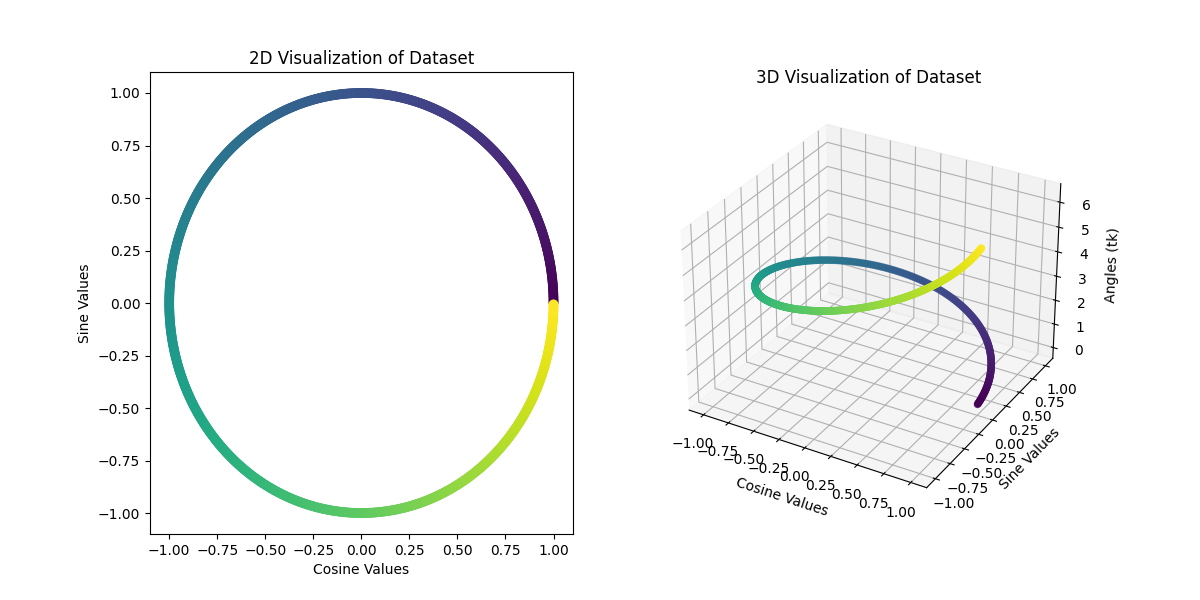
\includegraphics[width=0.7\textwidth]{images/ex3_task2_part1_dataset.png}
    \caption{Dataset of 1000  points}
    \label{fig:task1_dataset_fig}
\end{figure}

\textbf{Bonus: } On inspecting the plots, we can see that the first eigenfunction is constant. This eigenfunction corresponds to the eigenvalue with the largest magnitude and likely captures that overall trend or structure of the data which is similar to Fourier analysis, where the constant eigenfunctions resembles the main part of the signal. The subsequent eigenfunctions are sinusoidal which can be compared with the sinusoidal components in Fourier Analysis.\\
\begin{figure}[h]
    \centering
    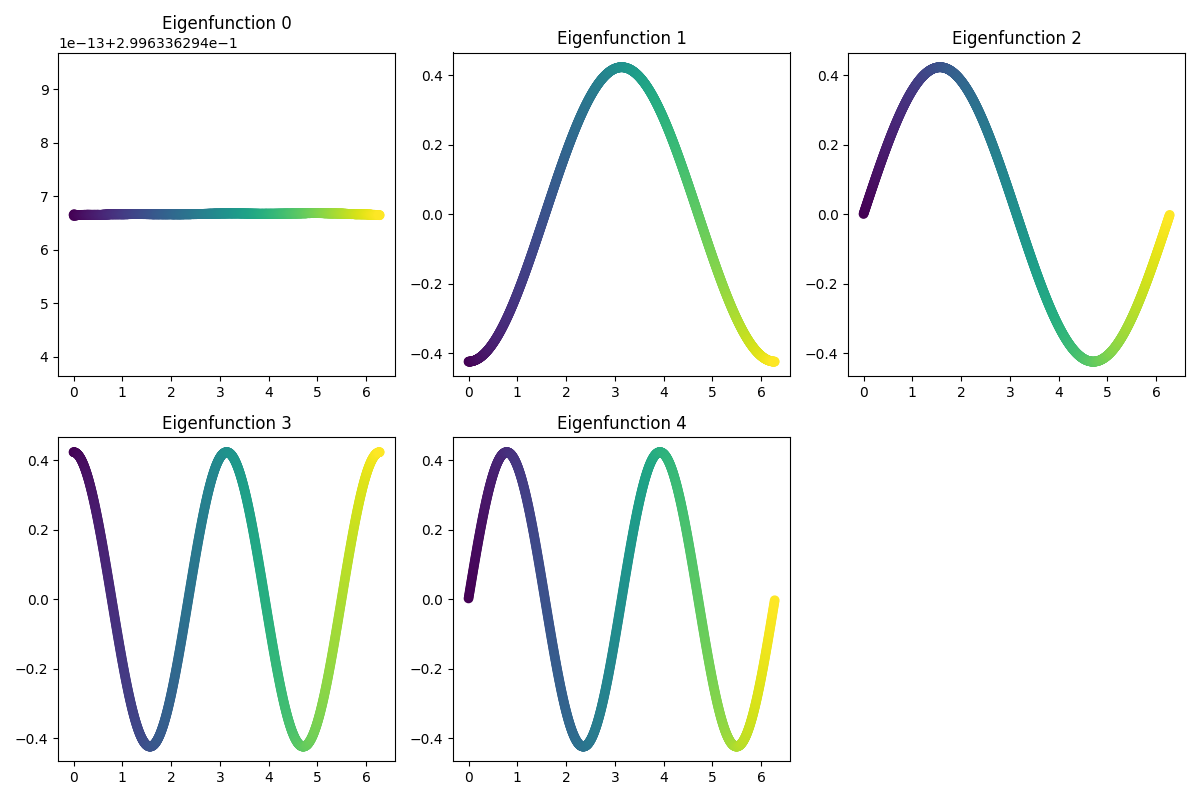
\includegraphics[width=0.6\textwidth]{images/ex2task1-1-2.png}
    \caption{Eigenfunctions associated to five largest eigenfunctions}
    \label{fig:eigenvalues_plotted}
\end{figure}




% P2: show a plot of the swissroll data in 3D.
\textbf{Part 2:} The Swiss roll dataset exemplifies a 2-dimensional (2D) manifold that is intricately rolled or curved within a 3-dimensional (3D) space. In general, a \( d \)-dimensional manifold can be understood as a subset within an \( n \)-dimensional space, where \( n \) is greater than \( d \). This manifold locally resembles a \( d \)-dimensional hyperplane. In the case of the Swiss roll, the dataset fundamentally represents a 2D plane, yet it exhibits a complex, rolled structure in 3D space. This characteristic makes it a particularly interesting case for studying dimensionality reduction techniques and manifold learning. We used the \texttt{make\_swiss\_roll()} function of the \texttt{sklearn.datasets} library to create a Swiss roll of 5000 points as shown in Figure \ref{fig:swiss_roll_5000}.\\

\begin{figure}[H]
    \centering
    \includegraphics[width=0.6\textwidth]{images/ex3\_task2\_swissRoll5000.png}
    \caption{Swiss roll with 5000 datapoints}
    \label{fig:swiss_roll_5000}
\end{figure}

% P2: 10 eigenfunctions on swiss roll, plotted against $\phi$1.
% P2: Number l of eigenfunctions where $\phi$l is no longer a function of $\phi$1?.
We used the implemented \texttt{Diffusion Map} algorithm to obtain approximations of the eigenfunctions associated with the swiss roll. We then plotted the first non-constant eigenfunction $\phi_1$ against the other eigenfunctions in 2D as shown in figure \ref{fig:task2.21}. Inspecting the plots we can see that the $\phi_0$ value is constant with respect to $\phi_1$. This aligns with the nature of the eigenfunctions where $\phi_0$ often represents the constant term capturing the overall trend or behaviour of the data. The values $\phi_2$,$\phi_3$, and $\phi_4$ appear to be dependent on $\phi_1$ as can be seen by the patterns in their plots. However, if we look at the plot of $\phi_5$, it seems to be independent of $\phi_1$. This functional independence of $\phi_l$(l>=5) shows that these eigenfunctions capture more localized and finer details that are not strongly influenced by $\phi_1$. They become increasingly independent and orthogonal to lower-order eigenfunctions.\\

\begin{figure}[H]
    \centering
    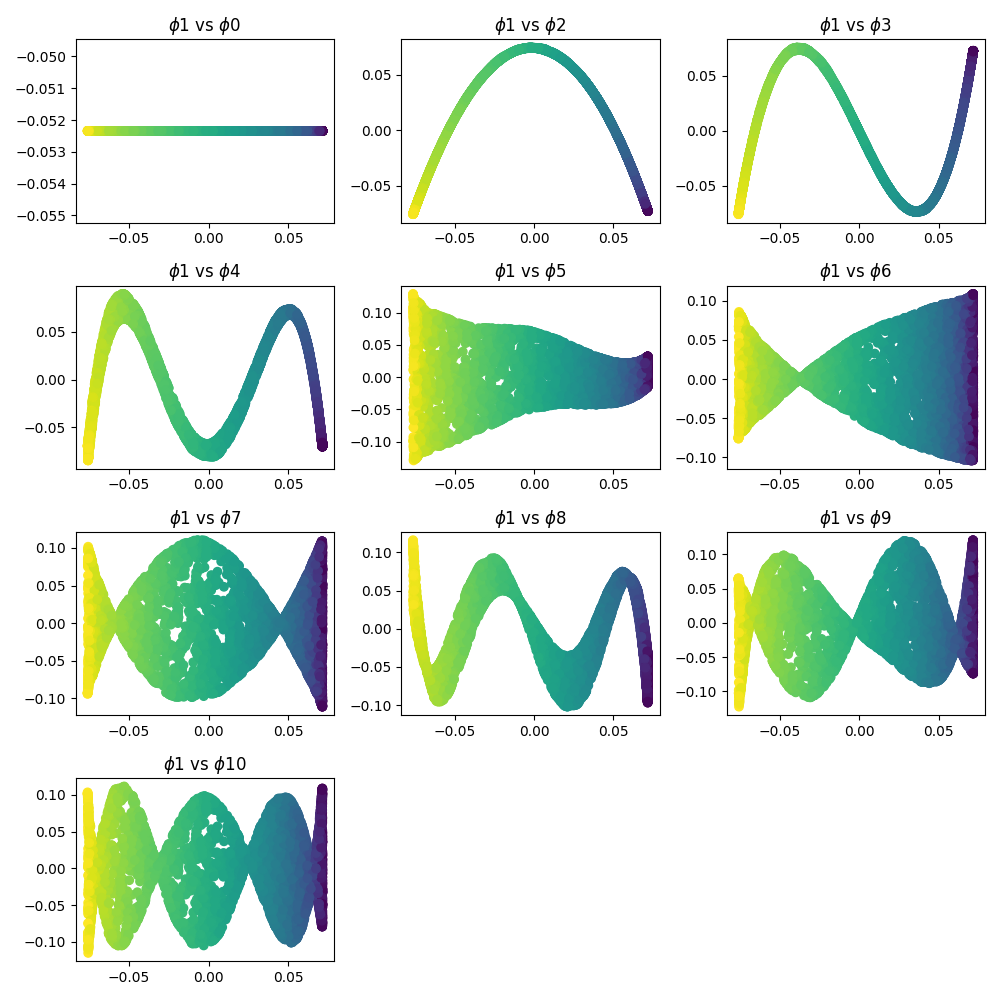
\includegraphics[width=0.6\textwidth]{images/ex3task2_5000vals.png}
    \caption{$\phi_1$ vs other $\phi$ values}
    \label{fig:task2.21}
\end{figure}


% P2: Why do you need three principal components for the swissroll, not two?
\textbf{PCA task:} Using the \texttt{PCA} implementation in task 1, we are now supposed to find the three principal components of the swiss-roll dataset. We can see that the \texttt{PCA Energy} is 100\% for this, meaning that we successfully captured the entirety of the dataset's information. However, if we investigate the \texttt{PCA Energy} related with only two principal components, we can observe a substantial reduction of nearly \texttt{29\%}. This reduction can be clearly seen in the plot of the reconstructed data as shown in figure \ref{fig:task2_PCA}. This indicates the loss in variance due to the absence of the third principal component which contributes vital information and omitting it leads to a significant loss of information and an inability to represent the data. \\

\begin{figure}[H]
\centering
    \begin{subfigure}{.4\textwidth}
        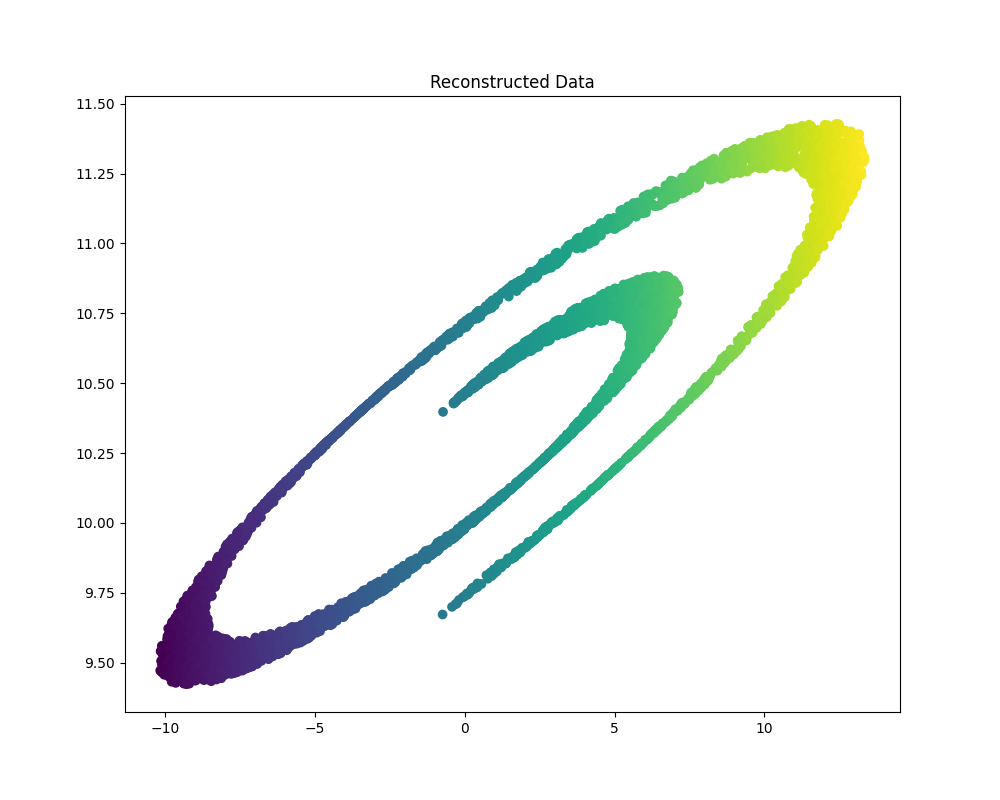
\includegraphics[width=\linewidth]{images/task2_reconstructedPCA.png}
        \caption{Reconstructed data with 2 PC}
        \label{fig:task2_PCA}
    \end{subfigure}
    \begin{subfigure}{.4\textwidth}
        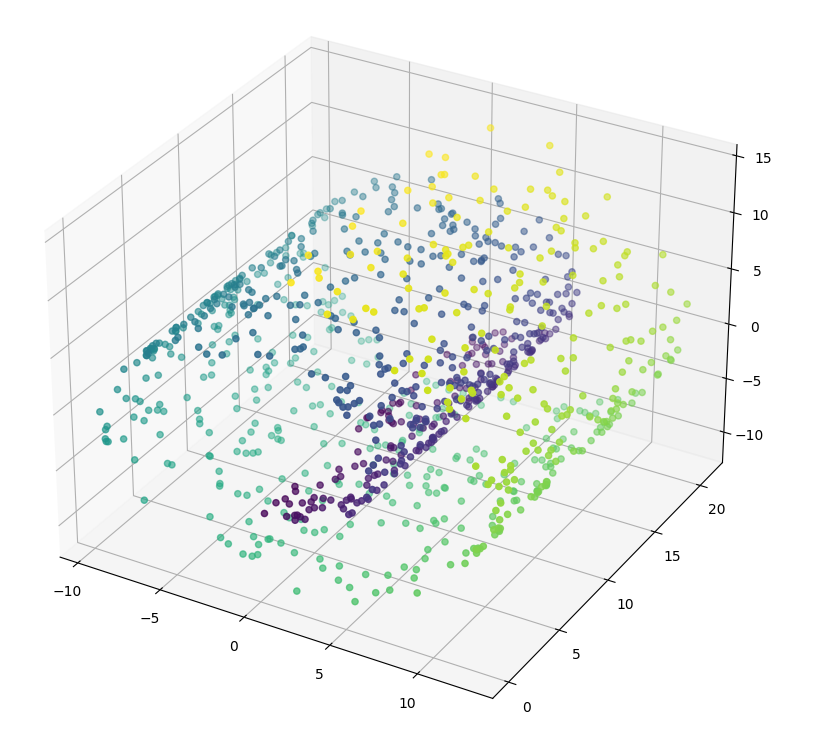
\includegraphics[width=\linewidth]{images/ex3task2_swissRoll1000.png}
        \caption{Swiss Roll with 1000 points}
        \label{fig:task2_Swiss_1000}
    \end{subfigure}
    
    \caption{}
    \label{fig:task2_PCA_1000}
\end{figure}
% P2: What happens with 1000 data points, for Diffusion Maps and PCA?
The next experiment was to reduce the number of data points from 5000 to 1000, as shown in figure \ref{fig:task2_Swiss_1000}. The dataset was again generated using the \texttt{make\_swiss\_roll} function. This dataset is much more sparse and less representative of the manifold. On repeating the experiment of plotting eigenfunctions calculated using \textit{Diffusion Maps}, we can clearly see in figure \ref{fig:task2.22} that they are much more noisy. This sparser dataset lacks the coverage required to represent the Swiss roll's complex geometry.

\begin{figure}[H]
    \centering
    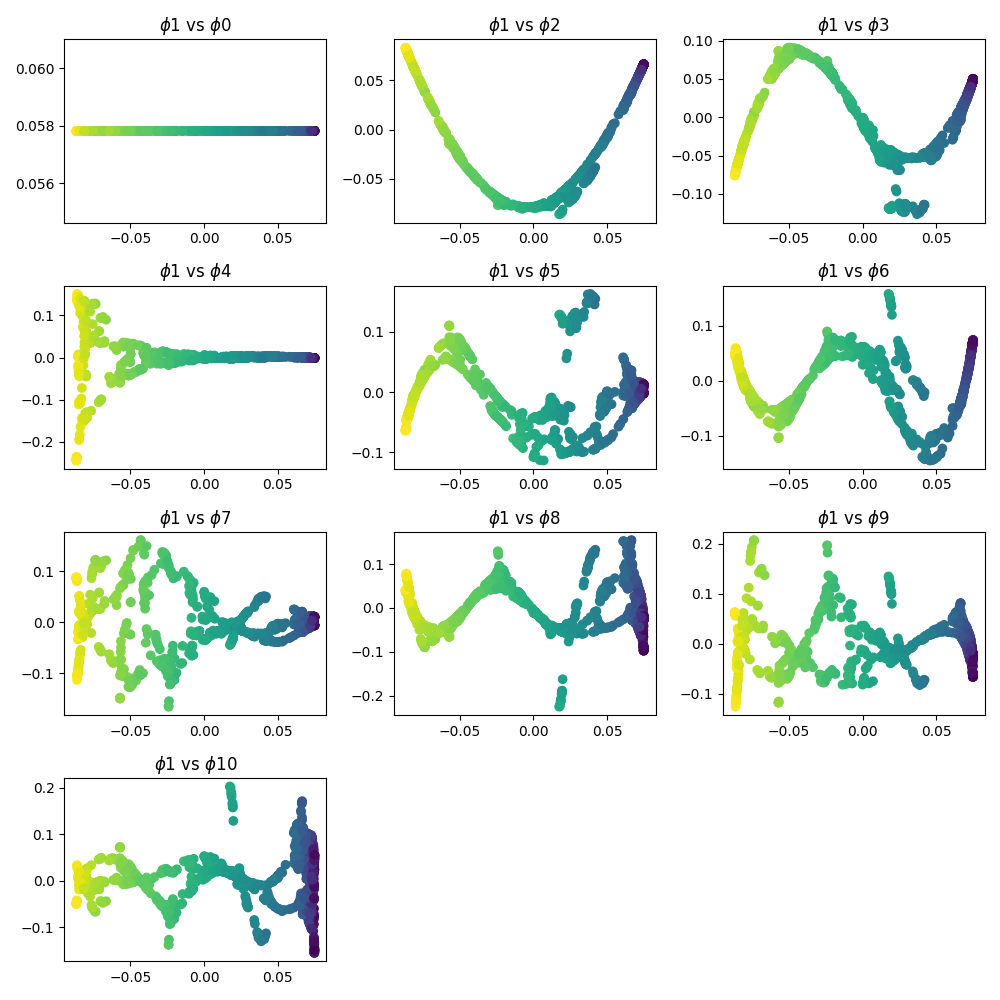
\includegraphics[width=0.8\textwidth]{images/ex3task2_1000vals.png}
    \caption{$\phi_1$ vs other $\phi$ values}
    \label{fig:task2.22}
\end{figure}

% P3: Same analysis as in PCA case for the file, but now with Diffusion Maps

\textbf{Part 3:} As described in the sheet, Diffusion Maps do not have the same exact energy interpretation of the eigenvalues (singular values) as PCA. Therefore, we started to check 3D graphs which consist of 3 consecutive eigenfunctions. It can be observed that for the 3D graph of $\Phi_1, \Phi_2, \Phi_3$, eigenfunctions can be used to fully unfold the data, which is not the case for the graph of the other triples, as can be seen in figure \ref{fig:task2_3_1}. 


If we further dig inside the graph of 2D consecutive eigenfunctions, we can observe that the graph of $\Phi_1, \Phi_2 $ eigenfunctions do not intersect. Hence it would be fair to say it is a proper embedding. If we check the other 2D graphs in figure \ref{fig:task2_3_2}, they all contain intersections in some ways. As $\Phi_1, \Phi_1 $ is also comparison with itself, we cannot consider that.


\begin{figure}[H]
\centering
    \begin{subfigure}{.28\textwidth}
        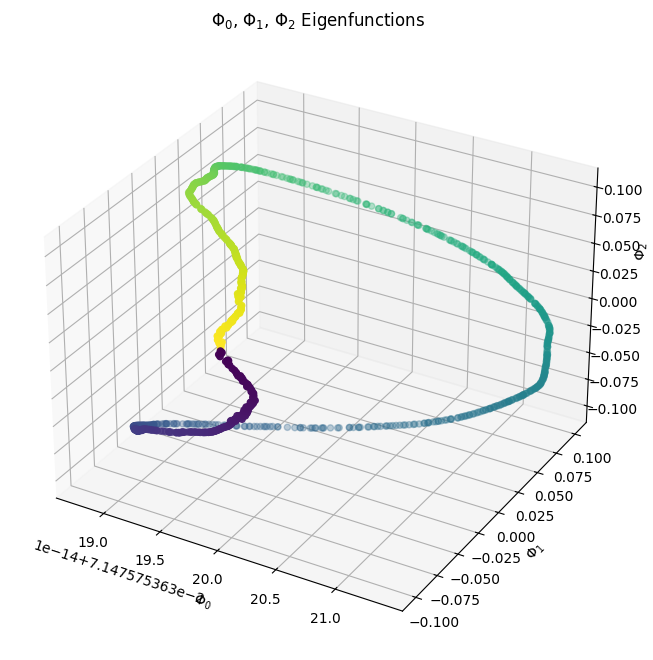
\includegraphics[width=\linewidth]{images/ex3_task2_part3_3D_1.png}
        \caption{$\phi_0, \phi_1, \phi_2$}
    \end{subfigure}%
    \begin{subfigure}{.28\textwidth}
        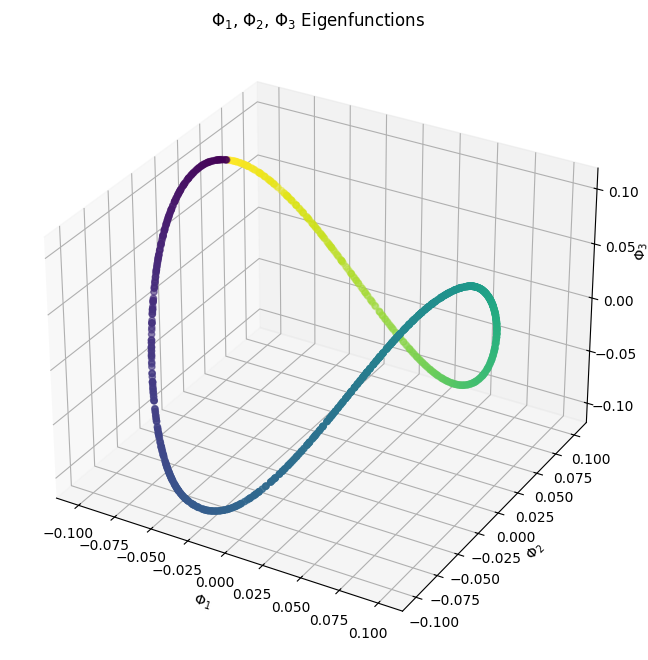
\includegraphics[width=\linewidth]{images/ex3_task2_part3_3D_2.png}
        \caption{$\phi_1, \phi_2, \phi_3$}
    \end{subfigure}%
    \begin{subfigure}{.28\textwidth}
        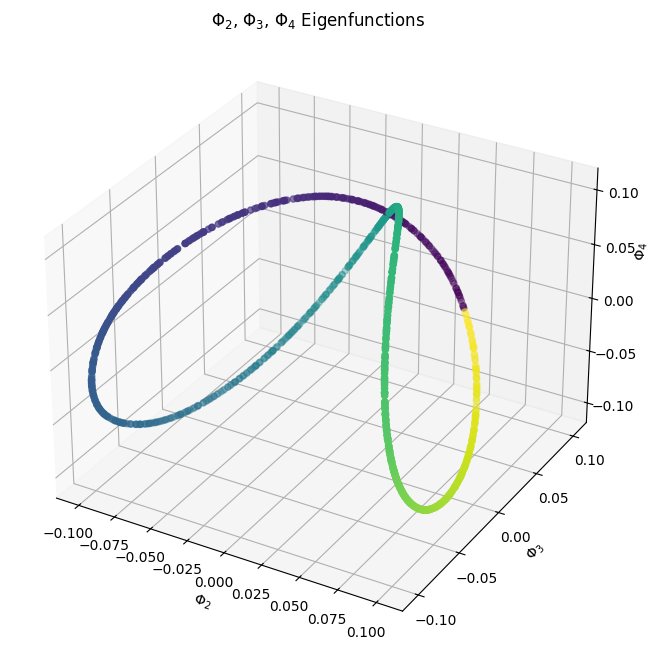
\includegraphics[width=\linewidth]{images/ex3_task2_part3_3D_3.png}
        \caption{$\phi_2, \phi_3, \phi_4$ }
    \end{subfigure}

    \medskip

    \begin{subfigure}{.28\textwidth}
        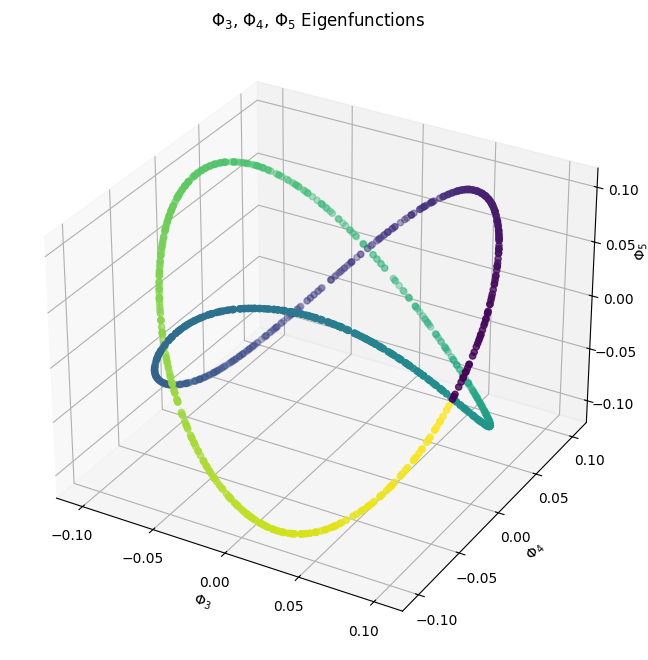
\includegraphics[width=\linewidth]{images/ex3_task2_part3_3D_4.png}
        \caption{$\phi_3, \phi_4, \phi_5$ }
    \end{subfigure}%
    \begin{subfigure}{.28\textwidth}
        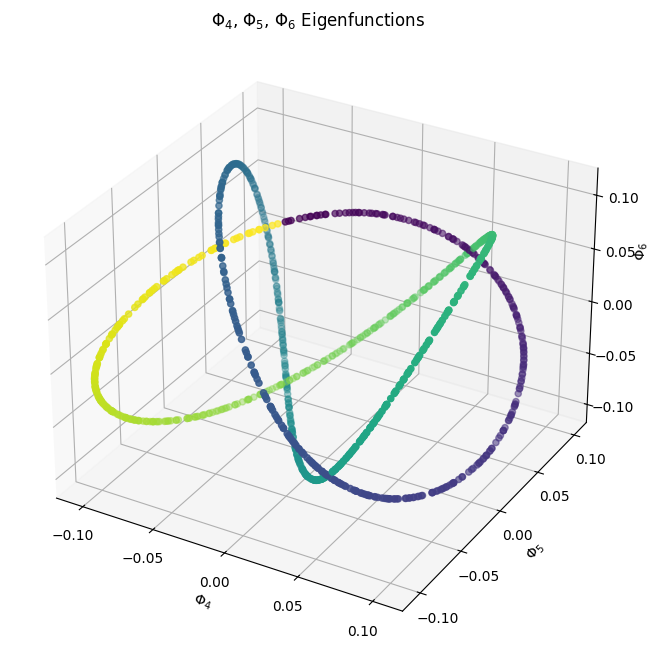
\includegraphics[width=\linewidth]{images/ex3_task2_part3_3D_5.png}
        \caption{$\phi_4, \phi_5, \phi_6$}
    \end{subfigure}%
    \begin{subfigure}{.28\textwidth}
        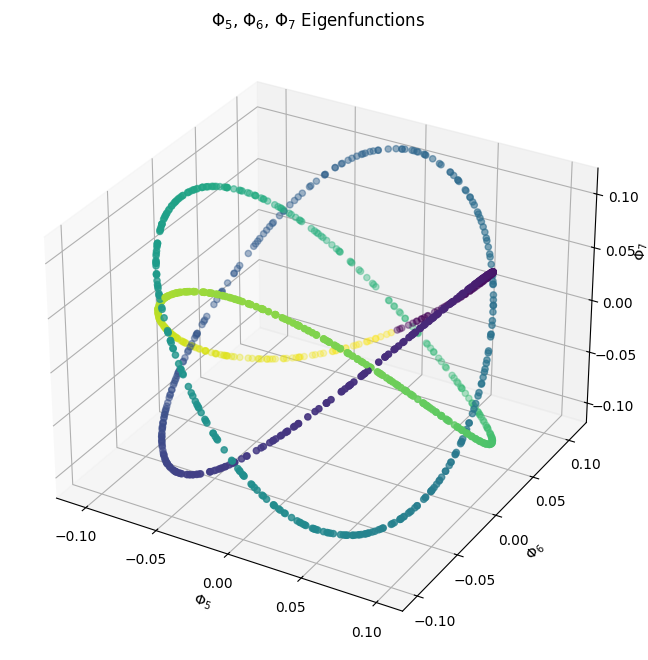
\includegraphics[width=\linewidth]{images/ex3_task2_part3_3D_6.png}
        \caption{$\phi_5, \phi_6, \phi_7$}
    \end{subfigure}
    
    \caption{Graphs for 3 Eigenfunctions in Euclidean Space}
    \label{fig:task2_3_1}
\end{figure}



\begin{figure}[H]
    \centering
    \begin{subfigure}{.25\textwidth}
        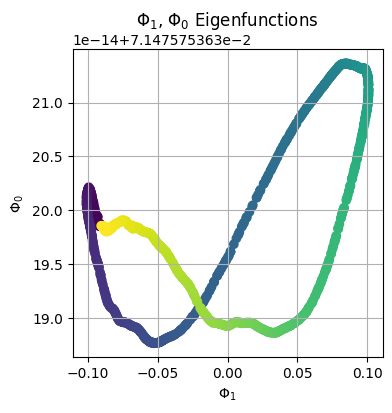
\includegraphics[width=\linewidth]{images/ex3_task2_part3_2D_1.png}
        \caption{$\phi_1, \phi_0$}
    \end{subfigure}%
    \begin{subfigure}{.25\textwidth}
        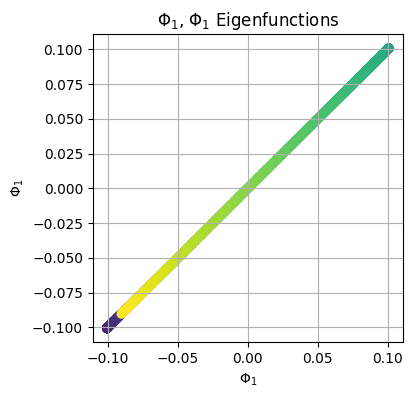
\includegraphics[width=\linewidth]{images/ex3_task2_part3_2D_2.png}
        \caption{$\phi_1, \phi_2$}
    \end{subfigure}%
    \begin{subfigure}{.25\textwidth}
        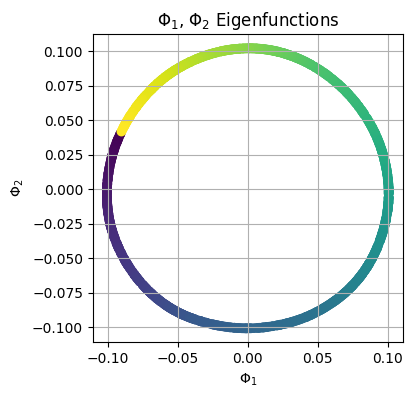
\includegraphics[width=\linewidth]{images/ex3_task2_part3_2D_3.png}
        \caption{$\phi_1, \phi_3$}
    \end{subfigure}
    
    \begin{subfigure}{.25\textwidth}
        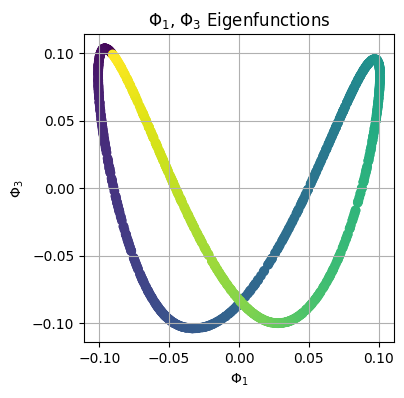
\includegraphics[width=\linewidth]{images/ex3_task2_part3_2D_4.png}
        \caption{$\phi_1, \phi_4$}
    \end{subfigure}%
    \begin{subfigure}{.25\textwidth}
        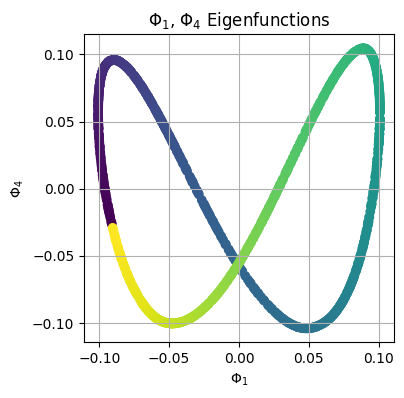
\includegraphics[width=\linewidth]{images/ex3_task2_part3_2D_5.png}
        \caption{$\phi_1, \phi_5$}
    \end{subfigure}%
    \begin{subfigure}{.25\textwidth}
        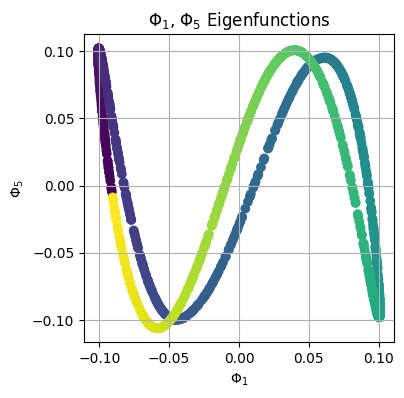
\includegraphics[width=\linewidth]{images/ex3_task2_part3_2D_6.png}
        \caption{$\phi_1, \phi_6$}
    \end{subfigure}
    
    \caption{Graphs for 2 Eigenfunctions in 2D Plane}
    \label{fig:task2_3_2}
\end{figure}


\textbf{Bonus task:} For this task, we are required to download the \texttt{datafold} library, which speacialize in manifold learning, and repeat the experiment on swiss roll dataset. The Swiss roll dataset has a very unique structure and lies on a curved manifold, therefore, PCA may not be able to provide an adequate low-dimensional representation. We followed the steps in the provided tutorial for s-curve manifold to compute and visualize the eigenvectors of the swiss roll. The code provided in the tutorial made it very easy to modify for swiss roll. The outputs generated by using the datafold library, as seen in figure \ref{fig:task2_datafold}, are consistent with the outputs generated by us. One of the main advantages that we observed by using the Datafold library was its high level of optimization. The library provided results in significantly less time compared to our previous implementation. The library also provides the function \texttt{LocalRegressionSelection} for automatic selection of optimal lower-dimensional embeddings which is a complex task, especially for high-dimensional data.



\begin{figure}[H]
    \centering
    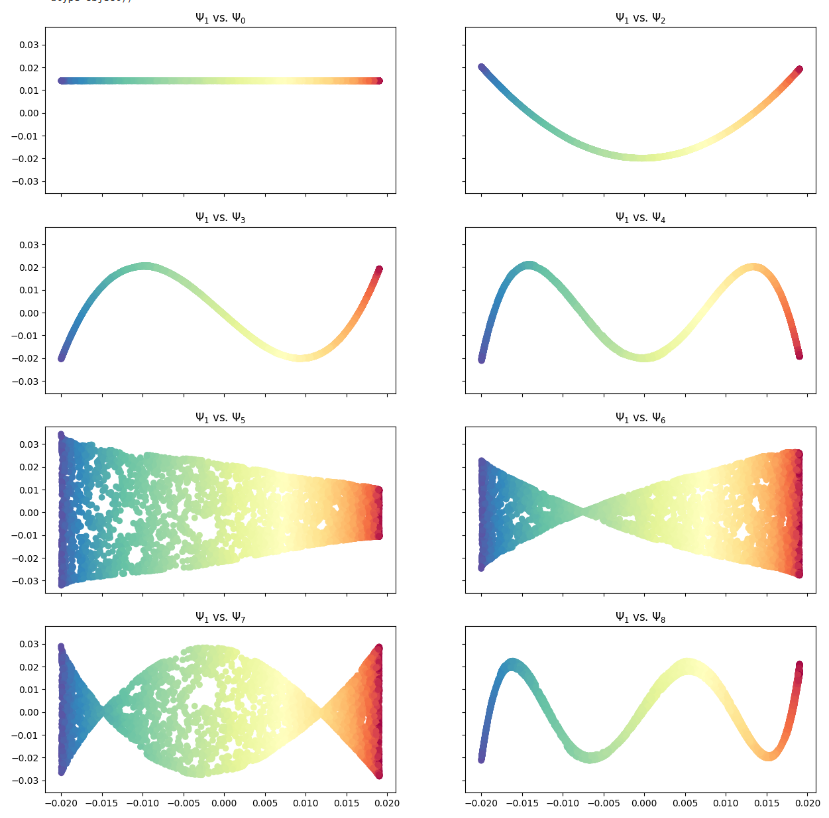
\includegraphics[width=0.6\textwidth]{images/ex3task2_datafold.png}
    \caption{$\phi_1$ vs other $\phi$ values generated using datafold}
    \label{fig:task2_datafold}
\end{figure}


% time estimate
% accuracy
% what we learned

% Verbose discussion of the results in the report?
% Code: modular, concise, well documented?
% Bonus: Verbose discussion of the datafold results in the report?